\documentclass[conference]{IEEEtran}
\usepackage{amsmath}
\usepackage{caption}
\usepackage{subcaption}
\usepackage{graphicx}
\usepackage{tikz}
\usepackage{algorithm}
\usepackage{algpseudocode}
\usepackage{graphicx}
\usepackage{float}
\usepackage{subfig}
\floatstyle{boxed}
\restylefloat{figure}
\ifCLASSINFOpdf
   \usepackage[pdftex]{graphicx}
  % declare the path(s) where your graphic files are
  % \graphicspath{{../pdf/}{../jpeg/}}
  % and their extensions so you won't have to specify these with
  % every instance of \includegraphics
  % \DeclareGraphicsExtensions{.pdf,.jpeg,.png}
\else
  % or other class option (dvipsone, dvipdf, if not using dvips). graphicx
  % will default to the driver specified in the system graphics.cfg if no
  % driver is specified.
  % \usepackage[dvips]{graphicx}
  % declare the path(s) where your graphic files are
  % \graphicspath{{../eps/}}
  % and their extensions so you won't have to specify these with
  % every instance of \includegraphics
  % \DeclareGraphicsExtensions{.eps}
\fi
% graphicx was written by David Carlisle and Sebastian Rahtz. It is
% required if you want graphics, photos, etc. graphicx.sty is already
% installed on most LaTeX systems. The latest version and documentation can
% be obtained at: 
% http://www.ctan.org/tex-archive/macros/latex/required/graphics/
% Another good source of documentation is "Using Imported Graphics in
% LaTeX2e" by Keith Reckdahl which can be found as epslatex.ps or
% epslatex.pdf at: http://www.ctan.org/tex-archive/info/
%
% latex, and pdflatex in dvi mode, support graphics in encapsulated
% postscript (.eps) format. pdflatex in pdf mode supports graphics
% in .pdf, .jpeg, .png and .mps (metapost) formats. Users should ensure
% that all non-photo figures use a vector format (.eps, .pdf, .mps) and
% not a bitmapped formats (.jpeg, .png). IEEE frowns on bitmapped formats
% which can result in "jaggedy"/blurry rendering of lines and letters as
% well as large increases in file sizes.
%
% You can find documentation about the pdfTeX application at:
% http://www.tug.org/applications/pdftex

\hyphenation{op-tical net-works semi-conduc-tor}


\begin{document}
\title{Automated Generation of Search-able PDF Format of Chemical Equations from Document Images}


\author{
\IEEEauthorblockN{Prerana Jana, Anubhab Majumdar, Sekhar Mandal}
\IEEEauthorblockA{Department of Computer Science and Technology\\
Indian Institute of Engineering Science and Technology Shibpur, 
India\\
Email: (prerana.jana, anubhabmajumdar93)@gmail.com\\sekhar@cs.iiests.ac.in}
\and
\IEEEauthorblockN{Bhabatosh Chanda}
\IEEEauthorblockA{Electronics and Communication Sciences Unit \\
Indian Statistical Institute, Kolkata,  India\\
E-mail : chanda@isical.ac.in}
}

%%%%%%%%%%%%%%%%%%%%%%%%%%%%%%%%%%%%%%%%

% make the title area
\maketitle

%%%%%%%%%%%%%%%%%%%%%%%%%%%%%%%%%%%%%%%%

\begin{abstract}
%\boldmath
The abstract goes here.
\end{abstract}

%%%%%%%%%%%%%%%%%%%%%%%%%%%%%%%%%%%%%%%%

\section{Introduction}

Here goes the introduction and previous work

%%%%%%%%%%%%%%%%%%%%%%%%%%%%%%%%%%%%%%%%

\section{Proposed Work}

Major steps involved in the automated generation of search-able PDF format are i) Segmentation of displayed chemical equation; ii) Recognition of various chemical symbols present in chemical equations; iii) Optical character recognition of each reactant; iv) Auto correction of reactants and the chemical equation itself; v) Generation of chemical equation in search-able PDF format.

%\begin{itemize}
%
%\item[A.]
%Segmentation of displayed chemical equation
%\item[B.]
%Recognition of various chemical symbols present in chemical equations 
%\item[C.]
%Optical character recognition of each reactant
%\item[D.]
%Auto correction of reactants and the chemical equation itself
%\item[E.]
%Generation of chemical equation in searchable PDF format
%
%\end{itemize}

The details of the above steps are given in the following subsections.

\subsection{Segmentation of displayed chemical equation}

Segmentation of displayed equations and then extracting only the chemical equations from a document image has been done using the methodology proposed in [1]. 
\subsubsection{Text Line Segmentation}

We have taken the horizontal projection profile of the document image to segment
the text line. The image and its horizontal projection profile is shown in Fig.\ref{fig:line segmentation}.

\begin{figure}[!h]\center\footnotesize
\begin{tabular}{|c|c|}\hline
 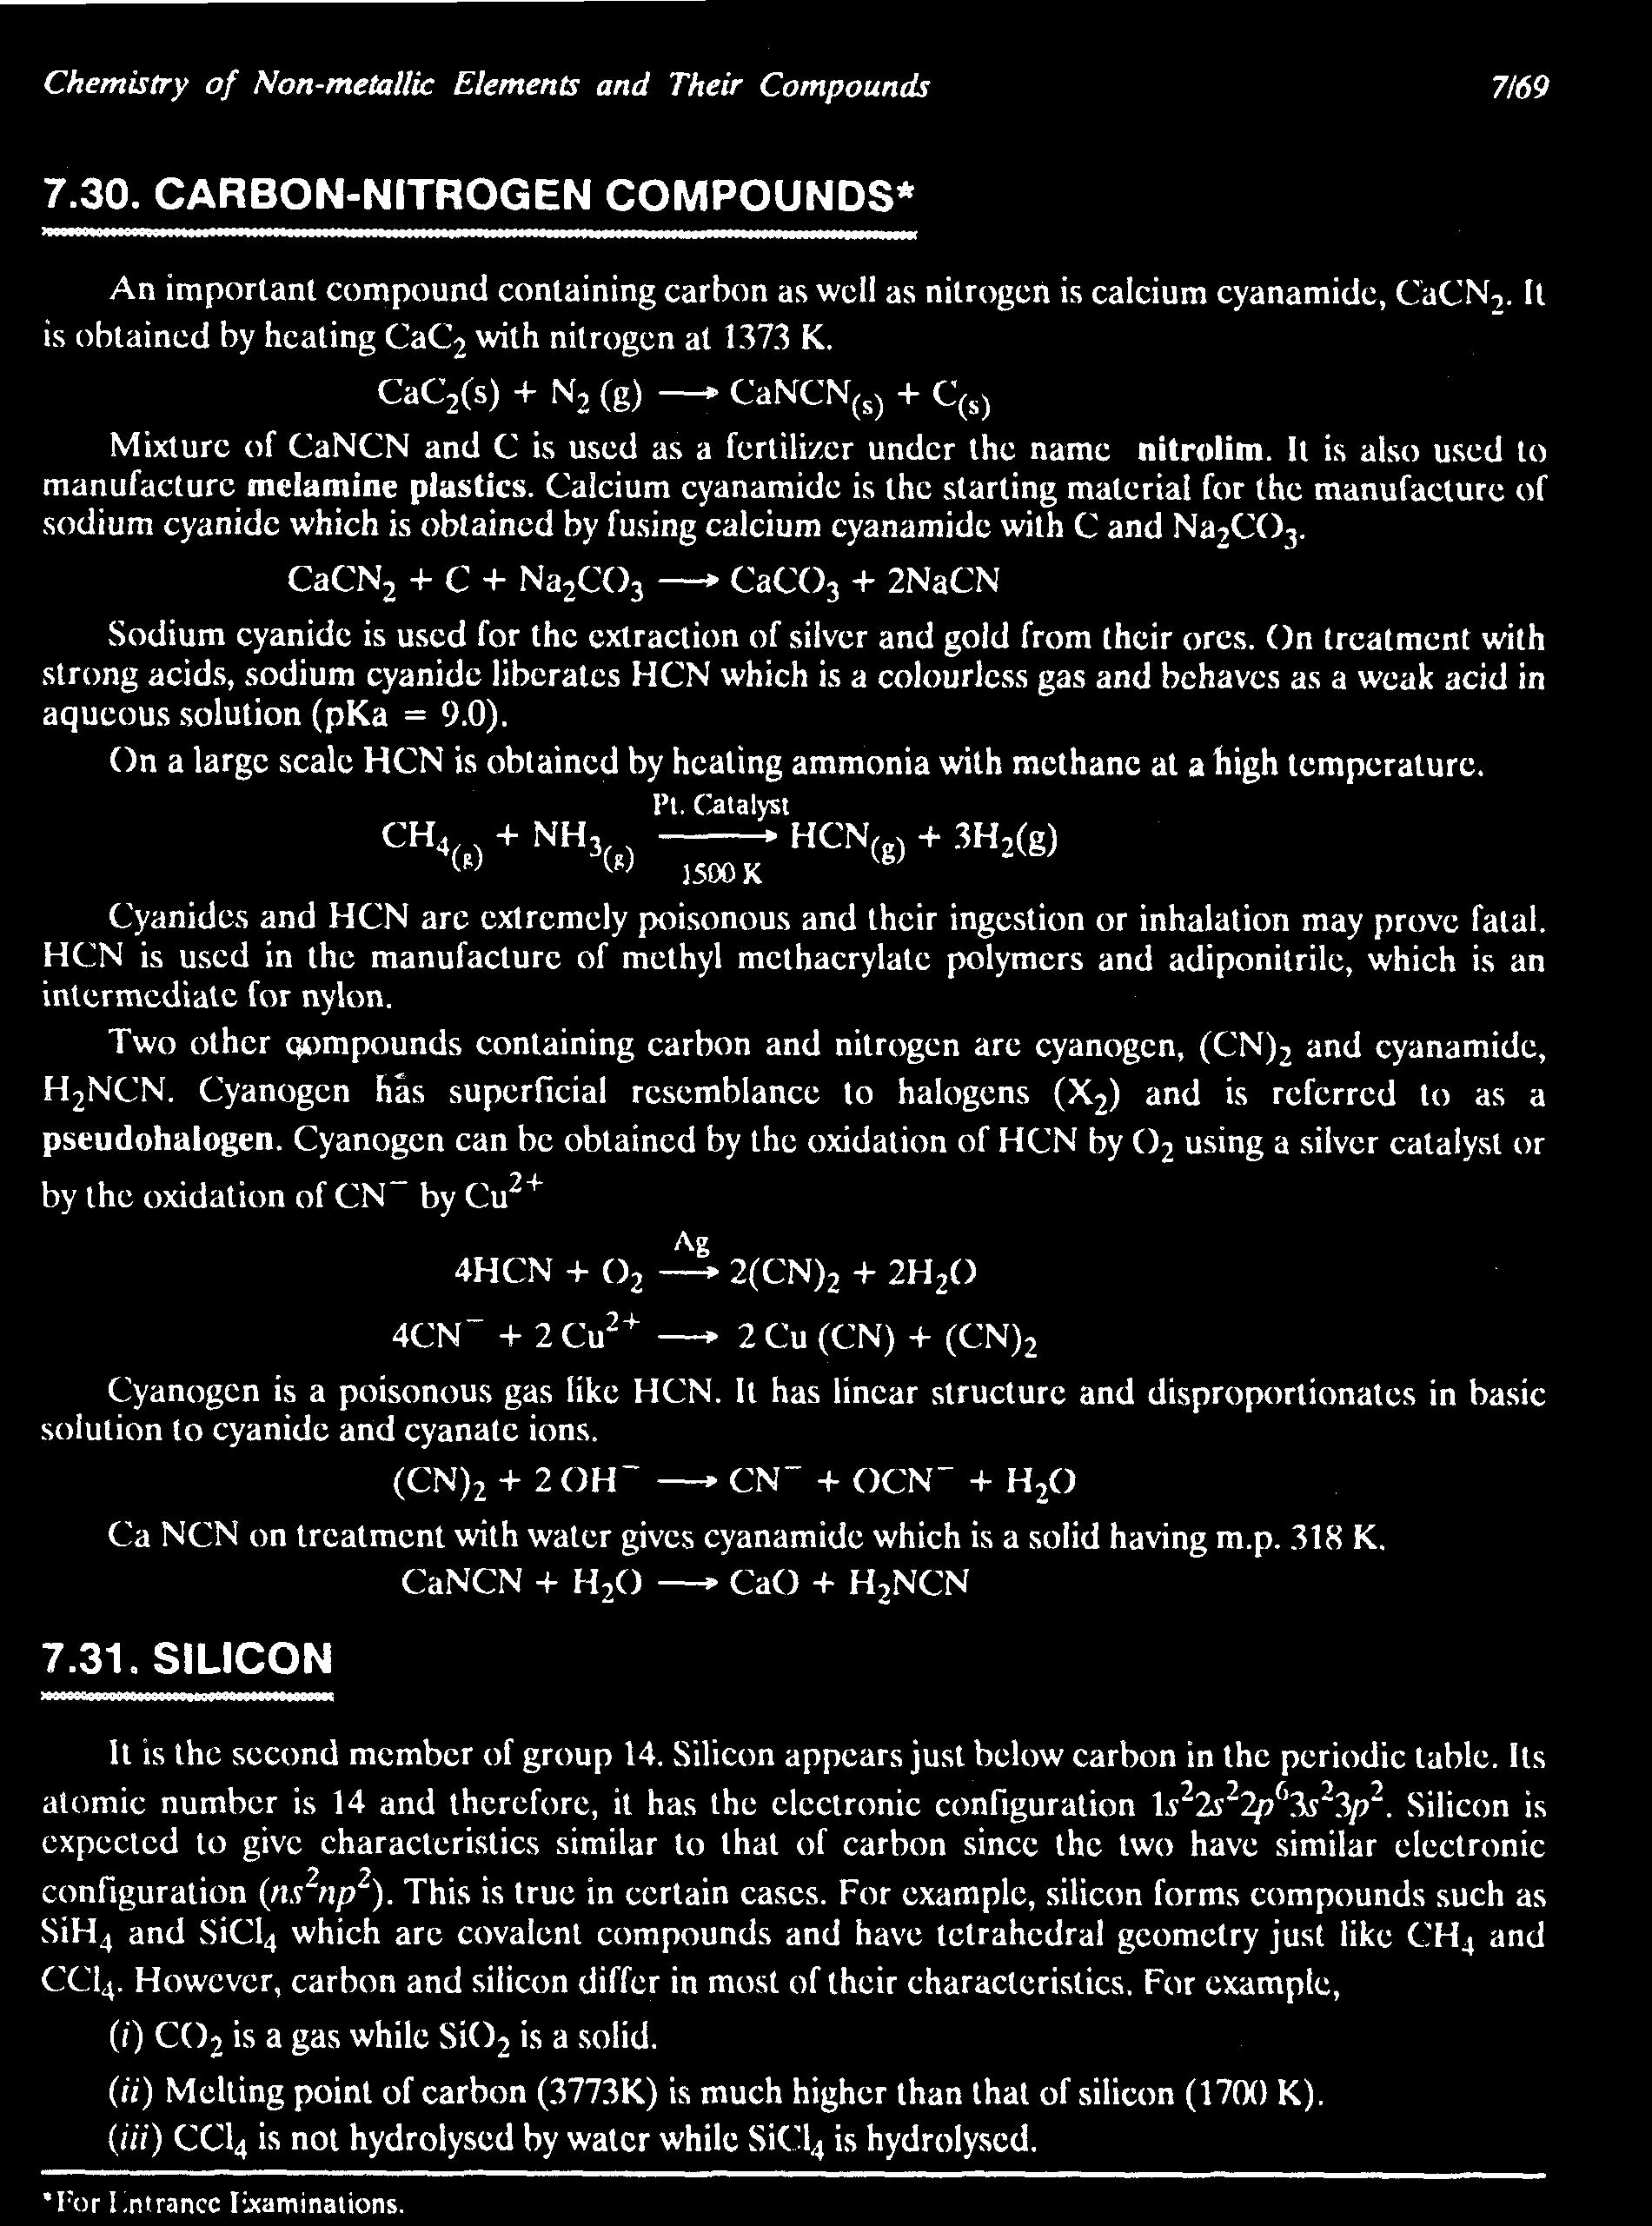
\includegraphics[width=0.35\linewidth]{sample_img.png} &  
 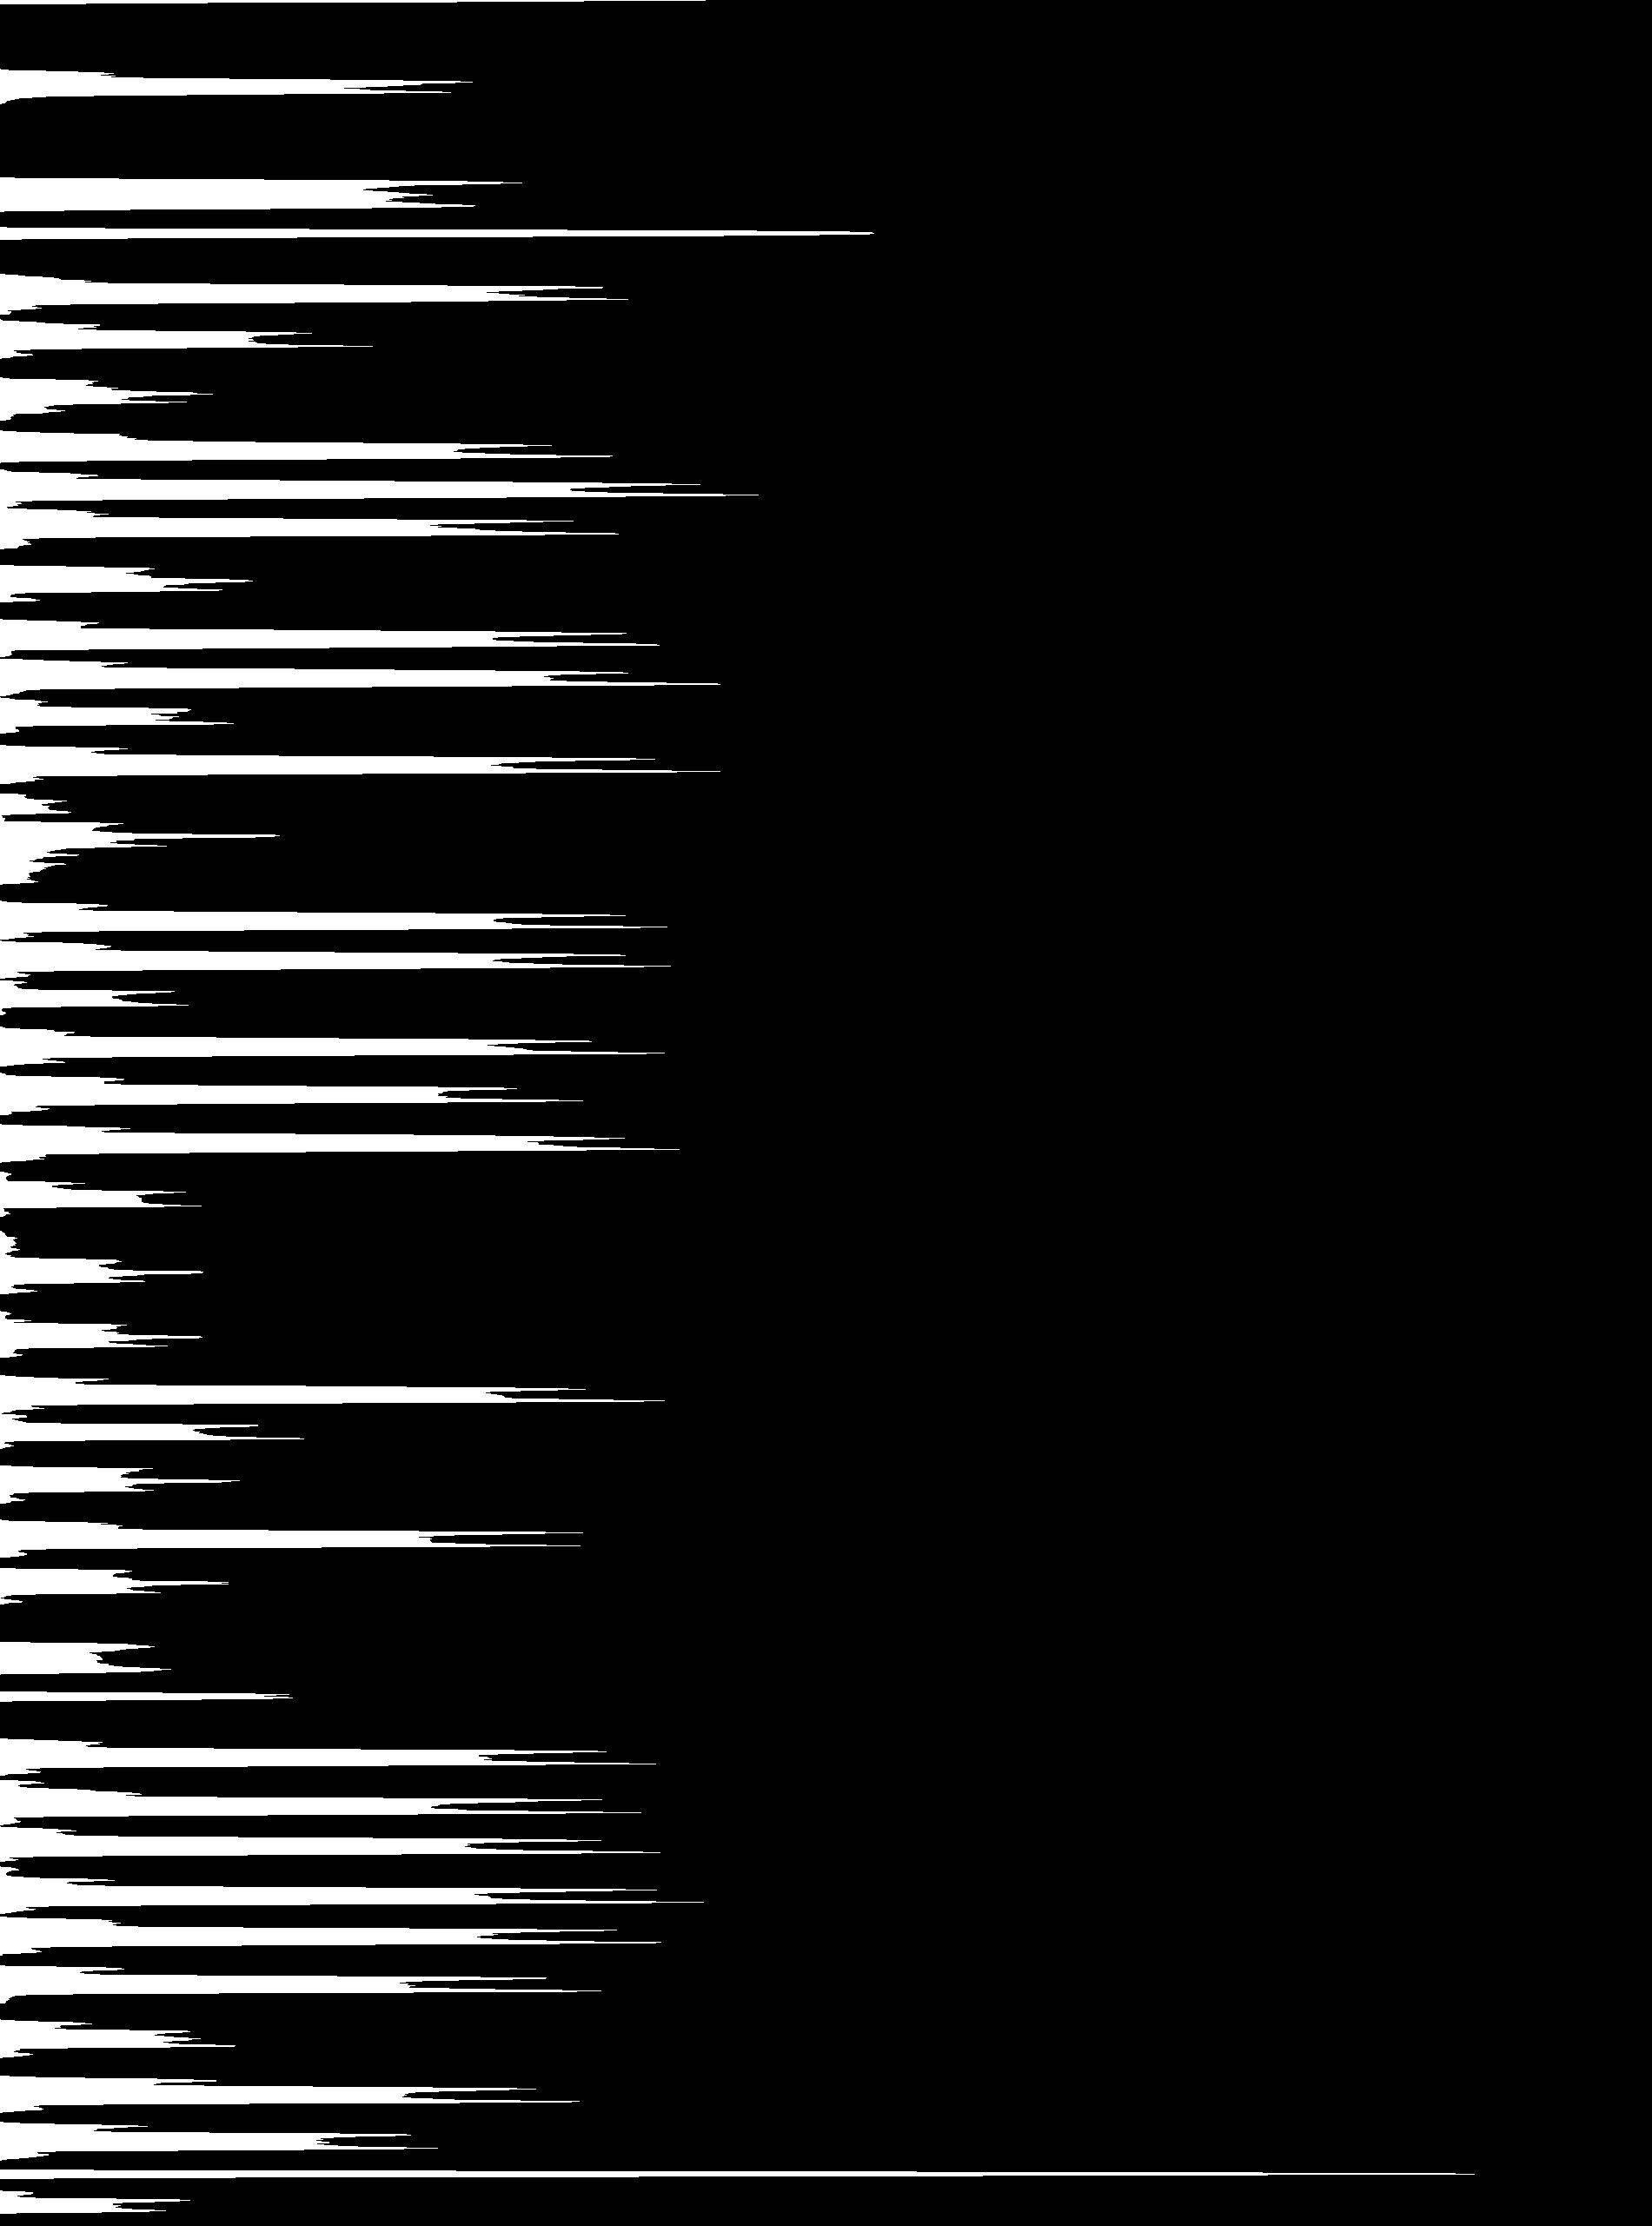
\includegraphics[width=0.35\linewidth]{h_proj.png}\\ 
 (a)&(b)\\ \hline
 \end{tabular} 
 \caption{(a). A scanned document image. (b). Horizontal projection profile.}
 \label{fig:line segmentation}
\end{figure}

Each disjoint component of Fig.1b is a line of the document image. This provides the bounding box coordinates of each line which is essential for segmentation.

\subsubsection{Word blob formation}

This requires performing morphological closing operation on the binary document image using a line structural element of suitable length. The length is determined by measuring white space between each adjacent component in the image and plotting the histogram. We will notice one high peak and a low peak separated by a valley which indicates the ideal structural element length. The high peak and low peak corresponds to gap between characters and gap between words respectively because statistically number of characters is much greater than number of words in a document. The histogram is shown in Fig.\ref{fig:histogram}. Therefore, the length of structural won't be greater than the gap between two words but certainly more than gap between two letters of a word.   
     
\begin{figure}[h]
\centering
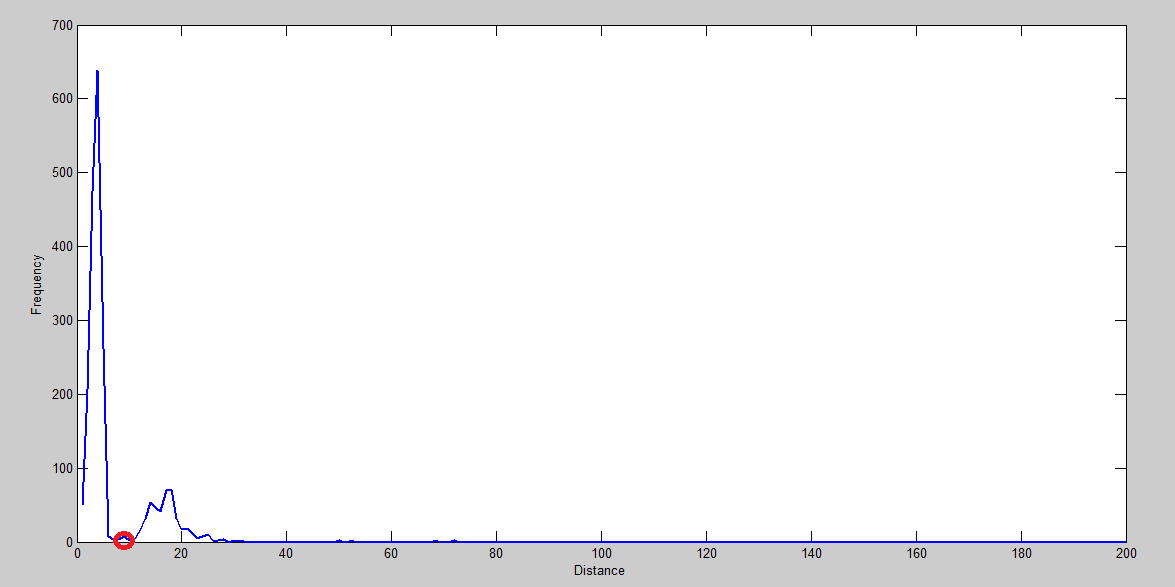
\includegraphics[width=0.9\linewidth]{histogram}
\caption{Histogram of white space between adjacent component. The red circle shows the ideal length of the structural element.}
\label{fig:histogram}
\end{figure} 

\subsubsection{Operator identification}

After formation of word blob, each component is labeled, the region corresponding to each component is considered and the number of connected component(s) in the region is counted. The chemical symbols we tried to identify are \{+, -, $\rightarrow$, $\leftarrow$, $\rightharpoonup$, $\leftharpoondown$, $\uparrow$, $\downarrow$\} and their blob will have one connected component only. Also these symbols will have Euler number 1. Using these rules we can filter out most words and few alphanumerics like 4, a, A etc. However along with the desired symbols few other symbols like (, ), \{, \} etc. will remain(see Fig.\ref{fig:singlechar}). An one class svm is used to classify the needed symbols from the unwanted(see Fig.\ref{fig:operator}). The feature vector used are:

\begin{itemize}
\item
Aspect ratio of each component.
\item
Density, i.e, $\dfrac{\#object_pixels}{\#background_pixels}$. 
\item
Horizontal and vertical projection profile for resized image is considered and for each profile the 2$^{nd}$ and 3$^{rd}$ order moment is computed.
\item
For each profile the location and magnitude global maximum is computed.
\item
The perimeter of the image.   
\end{itemize}
One class svm is used because the negative class is infinite. Its impossible to determine which character will remain as single character after removal using Euler number. 

\begin{figure}[h]

\begin{subfigure}{0.5\textwidth}
\centering 
\includegraphics[width=0.9\linewidth]{singlechar} 
\caption{}
\label{fig:singlechar}
\end{subfigure}

\begin{subfigure}{0.5\textwidth}
\centering 

\includegraphics[width=0.9\linewidth]{operator}
\caption{}
\label{fig:operator}
\end{subfigure}
 
\caption{(a). Single characters after removal using Euler number. (b). After classification using one class svm.}
\label{fig:image3}

\end{figure}

\subsubsection{Segmentation of Displayed Equations}

The lines having at least one symbol identified from the step above are either in line or displayed equation. To determine the displayed equation we use the blobbed image. We count the number of operators and operand in a line and identify a line as Displayed Equation(DE) if \#operands $\leq$ 2 x \#operands since a operator can have at most 2 operands on its either side. 

\subsubsection{Classification of segmented DE zones}

A hash-map of all the periodic element is made. The chemical symbol of all periodic element follows the regular expression [A-Z][a-z]$^{*}$. For each operand in DE, we take each connected component and input it in OCR. All substrings of a operand matching the regular expression are possible periodic elements and they are matched to the hash table. If $\dfrac{\#matches}{\#extracted} \geq$ 0.7, then we consider that DE as Displayed Chemical Equation(DCE). The reason for the ratio not being 1 are i) Limitations of OCR; ii) Touching and broken characters.  
  
\subsubsection{Improvements to proposed methodology in [1]}

Some improvements on the segmentation error has been attempted. 
For the reactants over the arrow, the main problem is single character extraction. In [1], component count has been done in the bounding box of one blob. Here, if we find multiple components, each component's bounding box is calculated. If one of the component's bounding box is equal to the bounding box of its blob, we remove the components with smaller bounding boxes  (See Fig.\ref{fig:arrow_error}). This is based on the positional context that an arrow with or without reactants over or below it will have the same bounding box as that of its word blob. 


\begin{figure}[h]\center\footnotesize
\begin{tabular}{c  c c }
%\hline 
 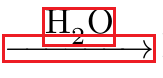
\includegraphics[width=0.3\linewidth]{arrow_with_element.png}&  
 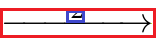
\includegraphics[width=0.3\linewidth]{segmentation_error.png}&  
 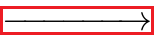
\includegraphics[width=0.28\linewidth]{segmentation_error_fixed.png} \\ 
(a)&(b)&(c)\\
 \end{tabular} 
 \caption{(a). Arrow with reactants over it. (b). Bounding Box of the arrow. (c). After removal of smaller components}
 \label{fig:arrow_error}
\end{figure}


\subsection{Recognition of various chemical symbols present in \\chemical equations} 
A chemical equation is a way of representing a chemical reaction in symbolic form.
Chemical equations consists of reactants separated by myriad chemical symbols. The symbols along with their significance are listed below. 

\begin{itemize}
\item
+ : Separates the reactants
\item
$\rightarrow$, $\leftarrow$ : Separates the reactants from products in irreversible reactions; also denote the direction of reaction
\item
$\leftrightarrow$, $\rightleftharpoons$ : Separates the reactants from products in reversible reactions
\item 
= : Shows stoichiometric equality in chemical equations
\item
$\uparrow$ : Used to denote gaseous compound
\item
$\downarrow$ : Used to denote sediments formed after a reaction
\end{itemize} 

We begin with the extracted displayed chemical equation (DCE) from the step above and run a HRLS algorithm. 
This results in the coalescing of the chemical compounds into a word blob as shown in Fig.\ref{fig:blob_equ}. 

\begin{figure}[h!]

\begin{subfigure}{0.5\textwidth}
\centering 

\includegraphics[width=0.9\linewidth]{original_equ} 
\caption{}
\label{fig:org_equ}
\end{subfigure}

\begin{subfigure}{0.5\textwidth}
\centering 

\includegraphics[width=0.92\linewidth]{blob_equ}
\caption{}
\label{fig:blob_equ}
\end{subfigure}
 
\caption{(a). Original DCE. (b). DCE after closing operation.}
\label{fig:image2}

\end{figure}

%The blobs with a singular component have a possibility for being a chemical symbol. However, it can also be a chemical element like C for Carbon, S for Sulphur or O for Oxygen as shown in Fig.\ref{fig:single_char_element}.
%


All the single components are identified and segregated from the original equation and classified using a decision tree shown in Fig.\ref{fig:decision_tree}.


The function of each node of the decision tree is detailed below.
\begin{itemize}
\item
\#of component : This module counts number of disjoint components in the input symbol.
\item
Crossing : We measure the number of transitions from object to background pixel and vice versa for each column while moving along the rows and consider the maximum value. 
\item
OCR : The input symbol is run through OCR to positively identify the + symbol. Other symbols return erroneous result.
\item
Aspect Ratio : Calculates the $\dfrac{height}{width}$ ratio of input image. 
\item
Distance Transform :  The input symbols are closed with a disc structuring element of radius $\frac{m}{2}$ where $m$ is $min(height,width)$ of the input symbol. The distance transform is applied and the location of the global maxima denotes the arrow head; hence determines the direction of the arrow.
\end{itemize}

\begin{figure}[h!]
\centering 
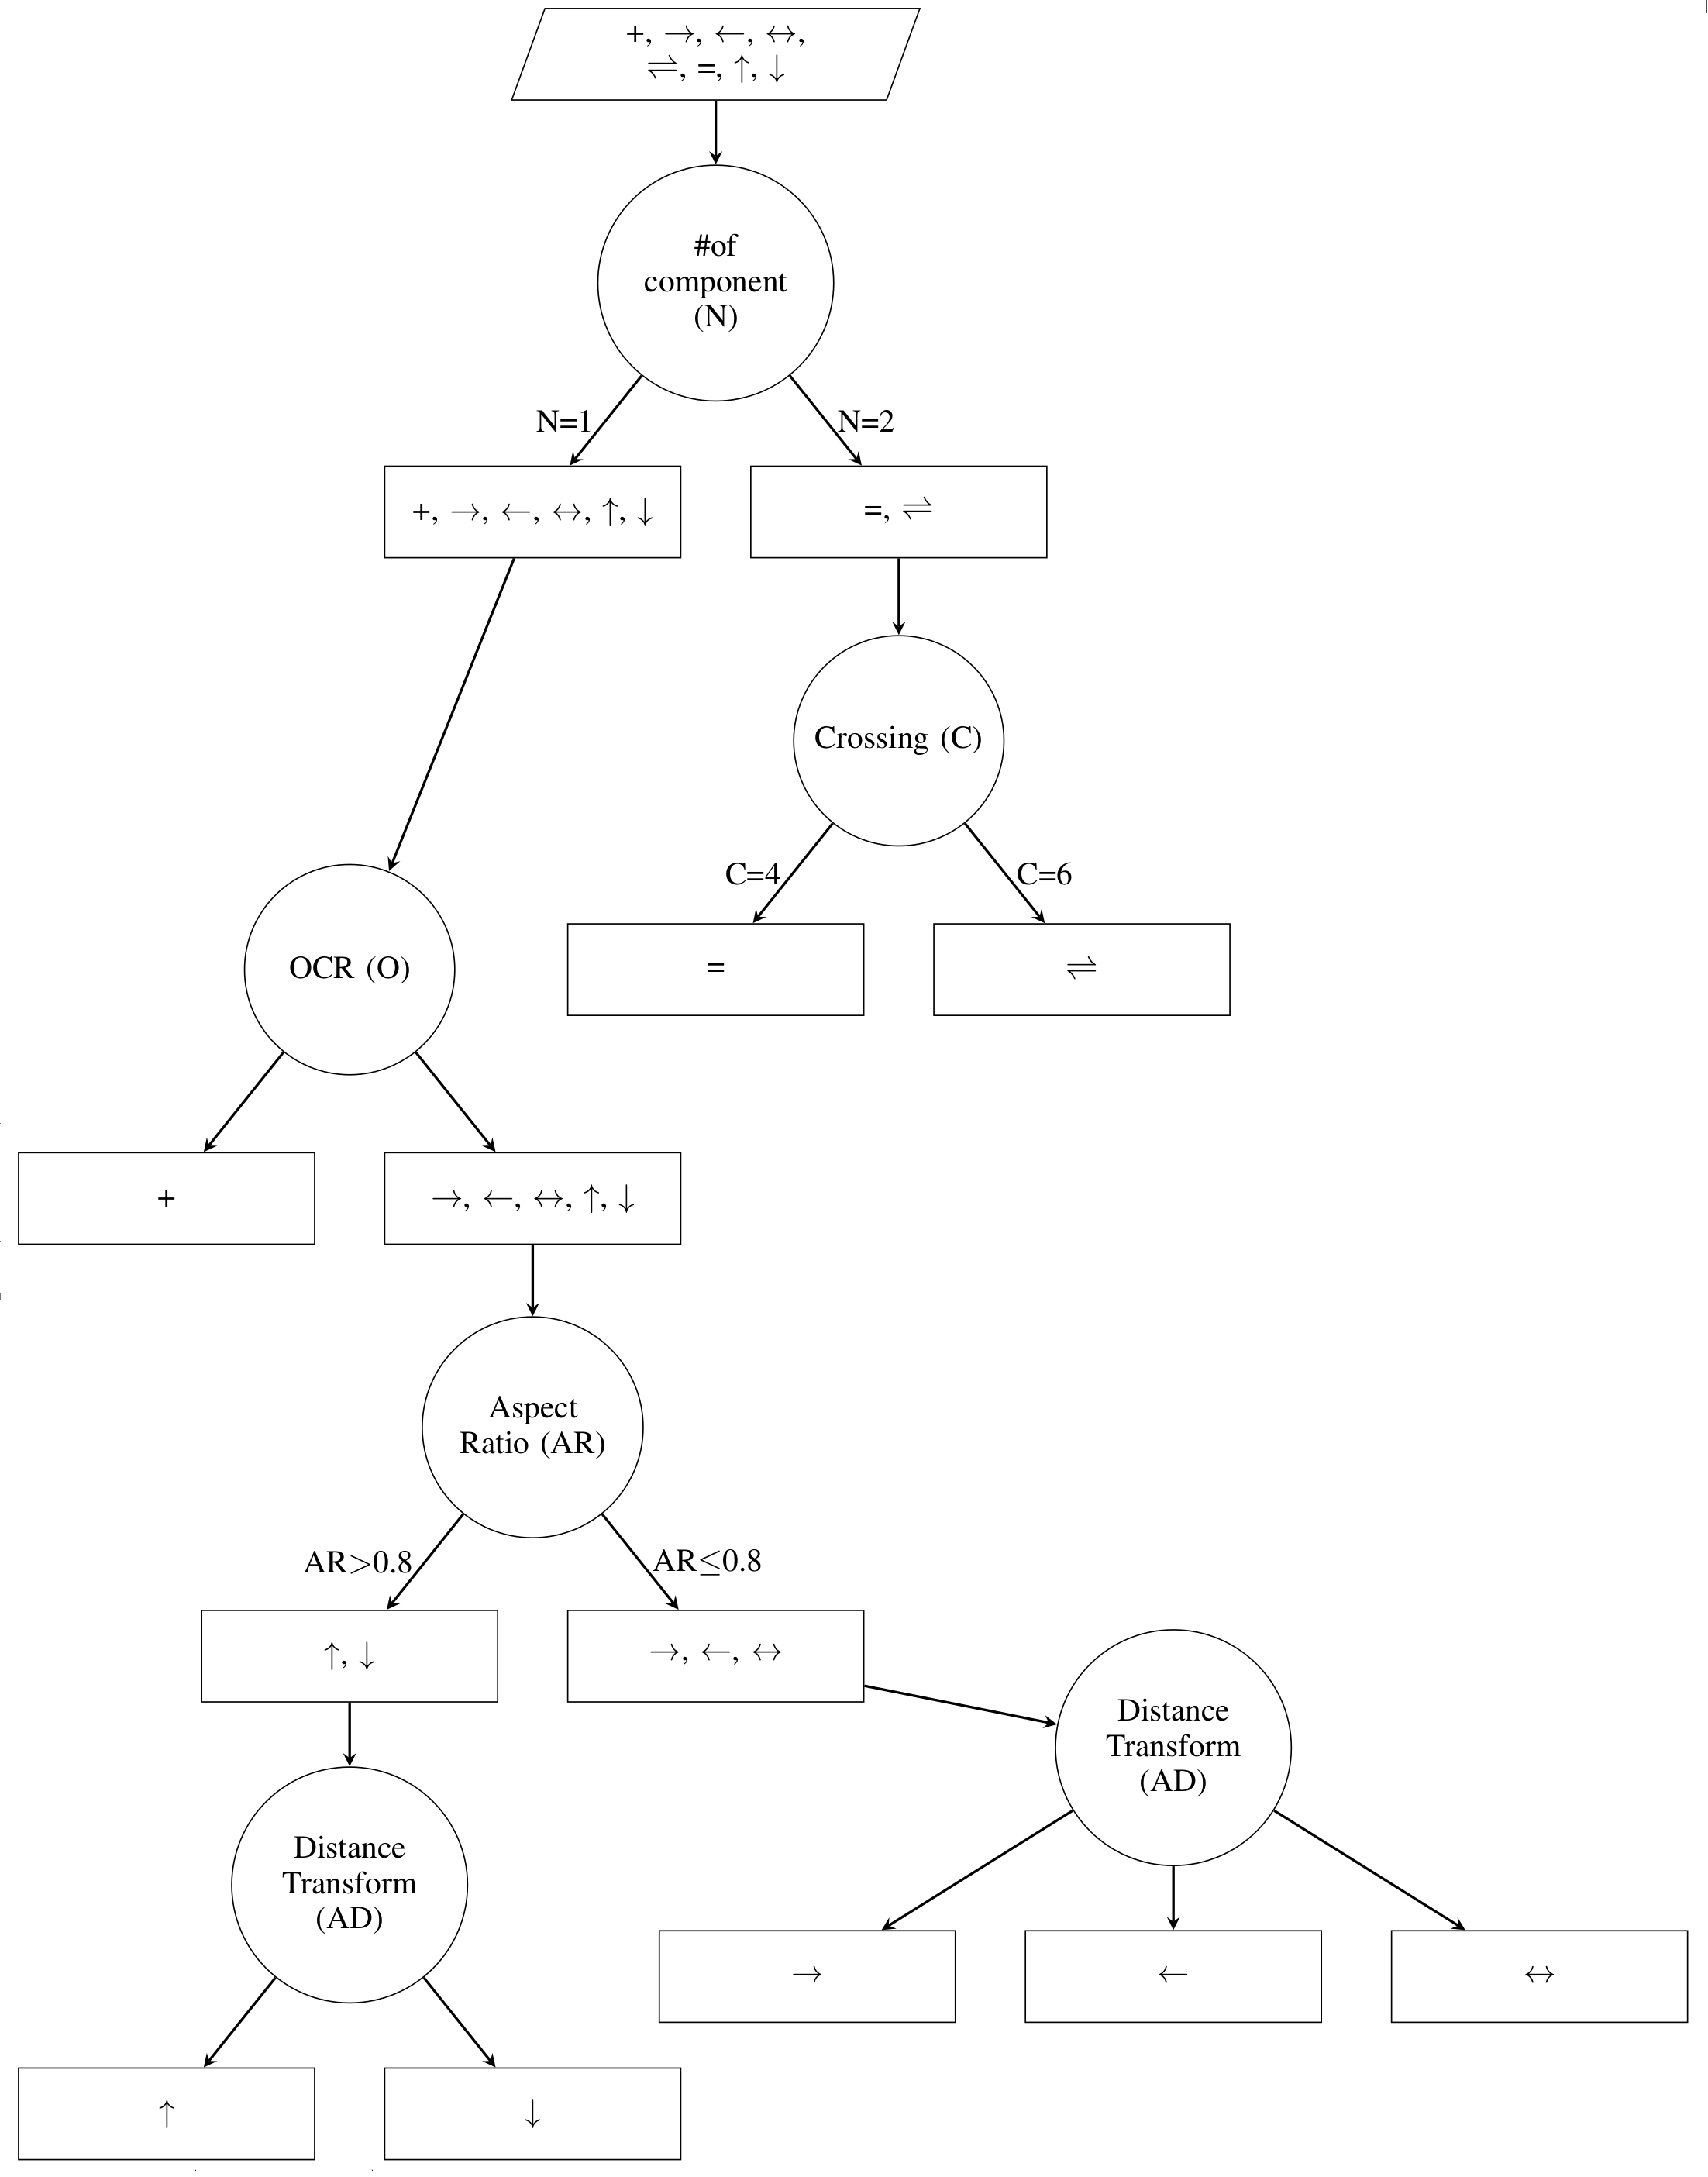
\includegraphics[width=0.95\linewidth]{decision_tree}
\caption{Decision Tree for Chemical Symbol Classification}
\label{fig:decision_tree}
\end{figure}

Certain chemical element like Carbon, Sulfur etc.(see Fig.\ref{fig:single_char_element}) may also be input to the tree and they get erroneously identified as $\uparrow$ or $\downarrow$ because characters have AR\textgreater0.8.
 
\begin{figure}[h!]
\centering

\includegraphics[width=0.9\linewidth]{single_char_element} 
\caption{DCE having element represented by single character}
\label{fig:single_char_element}
\end{figure}

To fix this, we match the symbols classified with the original equation blob image. For each +, $\rightarrow$,  $\leftarrow$, $\leftrightarrow$,  $\rightleftharpoons$ and = in the classified symbol set, we check its immediate right blob. If the blob has single component in the original equation image, then it must be an single character element because these symbols must be followed by reactants. Also the first blob is checked to see if its a single character element or not. 
Thus the chemical symbols are successfully segregated and classified from the chemical equation.
   
\subsection{Optical character recognition of each reactant}
After segregating the chemical symbols, rest of the blobs are considered as reactants. 
Each segment of a displayed chemical equation is divided into three zones; namely upper zone, middle zone and lower zone(see Fig.\ref{fig:supSub}). To identify the three zones of a DCE zone, uppermost and lowermost co-ordinates of each connected component below the same DCE zone are also obtained. The median of uppermost coordinate, and median of lowermost co-ordinate of such components in DCE zone are computed. A horizontal line, called the baseline, is drawn through the median of lowermost coordinates of components and this baseline separates the middle zone and lower zone of DCE zone. Similarly, the median of uppermost co-ordinate of the components in the DCE zone generates a horizontal line. This horizontal line, called top line, separates the middle and upper zones of the DCE zone. The subscripts in a DCE zone belong to lower-half of the middle zone and lower zone whereas the superscripts belong to upper zone and upper-half of the middle zone. Based on the location of the components in a DCE zone we have detected the subscripts and superscripts.
\begin{figure}[h!]
\centering
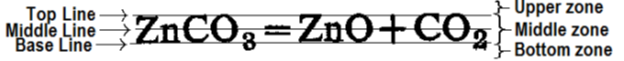
\includegraphics[width=0.9\linewidth]{supSub} 
\caption{Presence of different zones in DCE}
\label{fig:supSub}
\end{figure}
Each reactant form one word blob. Each character forming one word blob is run through an OCR engine, Matlab OCR. Each character image is returned by OCR engine in corresponding text format and saved in a string with a space split, S$_{reactant}$ for further processing. For each superscript and subscript, `\^{}'  and  `\_' are inserted before them respectively in S$_{reactant}$ for denoting purposes.
\subsection{Auto correction of reactants in chemical equations}
Matlab OCR does not give perfect result for chemical equations which has subscripts and superscripts as well. Hence, to generate the exact equation from the image, auto correction is required in chemical database. First an error map is created based upon our observation on multiple databases (see Table \ref{table:errorTable}). Next this table is stored into a hash map where the key is the OCR output and its corresponding value is possible input set. Auto correction is performed based on this error hash map, $H$.

Each chemical reactant in any equation has the following format-
[Coefficient]$^{[0,1]}$[Chemical compound][state]$^{[0,1]}$. Coefficient has numerical values, its regular expression is taken as [2-9]+[0-9]*. The first digit will not be 0 as coefficient cannot start with that. There are 4 states of a chemical compound which are represented by `(s)', `(g)', `(l)' and `(aq)'. To detect if the compound has any state representation, the following regular expression [(][a-z]$^{[1,2]}$[)] is checked in the substring of length 4 extracted from the end of S$_{reactant}$(blank spaces are ignored here). If there is a match, we run the autocorrection algorithm on it and compare the results with `s', `g', `l' and `aq'. If no match is found, the substring extracted from S$_{reactant}$ is a radical, not a state else, we remove the state from the reactant. After extracting coefficient and state, only chemical compound, $CC$ is left in S$_{reactant}$. So, $CC$ is a set containing OCR output of each character of the  chemical compound.


\begin{table}
\captionof{table}{Error list}
\begin{center}
 \begin{tabular}{|| c | c ||}
 \hline
 correct input & all observed outputs given by OCR\\
 \hline
 g & 8 3 S\\
 \hline
 n & l1 1'1 I1 11 X1 Il\\
 \hline
O & 0\\
\hline
3 & 8 'E s w \\
\hline
a & 3. 3 21 8 El 8. \\
\hline
q & Cl Q \\
\hline
H & 1-l 1-1 l-l l-1\\
\hline
2 & 7 4 Z z\\
\hline
l & 1 I\\
\hline
I & l\\
\hline
u & 11 U l1 ll 1l \\
\hline
i & 1 l I\\
\hline
5 & 'S \\
\hline
4 & A\\
\hline
Z & 2 \\
\hline
r & 1‘\\
\hline
e & C\\
\hline
s & S\\
 \hline
 \end{tabular}
 \end{center}
 \label{table:errorTable}
 \end{table}

The algorithm for autocorrection of each chemical compound is given below.
In first step, $CC$ and error map, $H$  are taken as input and all possible combinations of corrected OCR output is produced by $GetAllCombinations$. Next, these $Combinations$ are matched against a nearly exhaustive list of all molecules, chemical compounds, radicals and atoms named $ChemList$. If a perfect match is found, that is considered as the $Corrected$ chemical compound for that $CC$. But in case of no match, longest common substring(s) (LCS) between $Combinations$ and $ChemList$ are extracted and considered as $SubMatch$. If number of such $SubMatch$(es) is 1 that $SubMatch$ is considered as the $Corrected$ chemical compound for that $CC$; else they are considered as $PossibleReactants$. All the $Corrected$ compounds are included in the $FinalEquation$.
\begin{algorithm}
\caption{Auto-Correction of each reactant}
\begin{algorithmic}[1]
\Procedure {GetAllCombinations}{$CC$,$H$}
	\ForAll {$element(s) \in CC$}
		\State $InputSet(s) \leftarrow H.Get(element)$ 
		\If {$InputSet(s)$ is $NULL$}
			\State $RETURN$ \Comment Not in Error Map
		\Else
			\If {$length(element) = 1 $}
				%\State $InputSet =\cup$  $element $
				\State $InputSets =\cup$ $[element]$ 
				%\Comment Element might be correct output but still in the error list for other inputs
			\EndIf
		\EndIf
	\EndFor
\State $Combinations \leftarrow CartesianProduct(InputSets)$ %\Comment CartProd : Cartesian Product
\EndProcedure
\Statex

\Procedure {FindMatch}{$ChemList$,$Combinations$} %\Comment $ChemList$ : nearly exhaustive list of all molecules and chemical compounds
	\ForAll{$Combinations$}
		\State \textbf{match} {with $ChemList$}
	\EndFor
	\If {Match Found}
		\State $Corrected$ = Match
	\Else
		\State $SubMatch \leftarrow \textbf{LCS}(Combinations,ChemList)$ 
		\Statex \Comment LCS : Longest Common Substring
		\If {{NumberOf}($SubMatch$)=1}
			\State $Corrected = SubMatch$
		\Else
			\State $PossibleReactants \leftarrow SubMatch$
		\EndIf
	\EndIf

\EndProcedure
\end{algorithmic}
\end{algorithm}

Here we have all the possible reactants and try to find out the $FinalEquation$ in the context of the equation itself. Chemical equations have the same elements in the left hand side (LHS) as that in the right hand side (RHS). All the periodic elements follow the regular expression [A-Z][a-z]*. So, for each possiblity, the set of periodic elemnents in the left side of the equation,$P_{LHS}$ and in the right side, $P_{RHS}$ is computed. When the intersection of these two sets are empty, that $PossibleReactant$ is considered as $Corrected$ and included in the $FinalEquation$. But if the above condition comes true for multiple possibilities, we cannot decide which of the possible reactants are actually in the original equation.The algorithm shows multiple $FinalEquation$s. This is considered as an $ERROR$ case.\\

\begin{algorithm}
\caption{Auto-Correction of equation}
\begin{algorithmic}[1]
\Procedure {GetFinalEquation}{$PossibleReactants$}
	\For{every possibility}
		\State \textbf{compute}($P_{LHS}$)  
		\Statex \Comment{$P_{LHS}$ :  Set of periodic elements in the L.H.S}
		\State \textbf{compute}($P_{RHS}$)  \
		\Statex \Comment {$P_{RHS}$ : Set of periodic elements in the R.H.S}
		
		\If{$P_{LHS} \cap P_{RHS} = \emptyset $}
			\State $Corrected \leftarrow PossibleReactant$
			\State {Include that in the $FinalEquation$}
		\EndIf
	\EndFor
	\If {multiple possibilities get $P_{LHS} \cap P_{RHS} = \emptyset $ }
		\State {Multiple $Corrected$ compounds}
		\State{Multiple $FinalEquations$}
		\Statex \Comment { $ERROR$}
	\EndIf
\EndProcedure
\end{algorithmic}
\end{algorithm}


\subsection{Generation of search-able PDF format of chemical equations}

The operand list and chemical symbol list is used to form the auto corrected equation. We alternatively put a operand and a symbol starting with operand. Also, for each $\uparrow$ or $\downarrow$ in the symbol list, we put the next symbol from the list before placing another operand. After the list is formed, we write it in a Tex file with mhchem package. The Tex file is run later to generate the search-able PDF.   



%%%%%%%%%%%%%%%%%%%%%%%%%%%%%%%%%%%%%%%%

\section{Experimental Result}

Here goes the results.

%%%%%%%%%%%%%%%%%%%%%%%%%%%%%%%%%%%%%%%%

\section{Conclusion}
The conclusion goes here.





\begin{thebibliography}{1}

\bibitem{IEEEhowto:kopka}
H.~Kopka and P.~W. Daly, \emph{A Guide to \LaTeX}, 3rd~ed.\hskip 1em plus
  0.5em minus 0.4em\relax Harlow, England: Addison-Wesley, 1999.

\end{thebibliography}




% that's all folks
\end{document}


